\documentclass{article}

% ---------------------------------------------------------------------------
% NeurIPS 2024 style. neurips_2024.sty is bundled alongside this file, so the
% paper compiles on Overleaf or locally with no manual download. Use [preprint]
% while drafting; switch to the camera-ready/submission option at the venue we
% finally target.
% ---------------------------------------------------------------------------
\usepackage[preprint]{neurips_2024}

\usepackage[utf8]{inputenc}
\usepackage[T1]{fontenc}
\usepackage{hyperref}
\usepackage{url}
\usepackage{booktabs}
\usepackage{amsfonts}
\usepackage{amsmath}
\usepackage{nicefrac}
\usepackage{microtype}
\usepackage{graphicx}
\usepackage{xcolor}

% Draft note macro — strip before submission.
\newcommand{\todo}[1]{\textcolor{red}{[TODO: #1]}}
\newcommand{\prelim}[1]{\textcolor{blue}{#1}}

\title{Disentangling Statistical Surprisal from Hierarchical Structure\\
in LLM--Brain Alignment}

\author{%
  Sudarssan N.\thanks{Correspondence: \texttt{sudarssan73@gmail.com}} \\
  Independent Researcher \\
  \texttt{sudarssan73@gmail.com} \\
  \And
  Jeyaanth A. \\
  Independent Researcher \\
  \texttt{jeyaanth.am@gmail.com} \\
}

\begin{document}

\maketitle

\begin{abstract}
Large language model (LLM) hidden states linearly predict human language-network fMRI
responses at close to the noise ceiling, but it remains contested whether this alignment
reflects shared \emph{linguistic structure} or merely shared sensitivity to next-word
predictability (surprisal) and to low-level stimulus confounds. We quantify, on the Pereira
et al.\ (2018) benchmark, how much voxel-level alignment is \emph{uniquely} explained by LLM
hidden representations \emph{beyond} a controlled nuisance space, using cross-validated ridge
encoding combined with variance partitioning (commonality analysis). Crucially, our nuisance
space is not surprisal alone: it bundles surprisal, predictive entropy, word rate, word
length, word frequency, and \emph{sentence position}---the positional and word-rate signals
that recent work shows are competitive with trained LLMs on this dataset
\citep{feghhi2024}. Across eleven models spanning $70$M--$1.5$B parameters and four families,
the unique-hidden contribution \emph{survives} this strict control: adding the low-level
confounds to surprisal removes only $4$--$9\%$ of peak unique-hidden, which still exceeds the
unique contribution of the entire nuisance space by roughly an order of magnitude
($\sim$$7$--$15\times$) and grows with network depth. Using the Pythia suite as a confound-free
scaling axis ($70$M$\rightarrow$$1.4$B, identical data and training order), unique structure
rises with scale and saturates near $1$B. Instruction tuning \emph{significantly reduces}
unique-hidden at \emph{both} scales tested (Qwen2.5-0.5B and -1.5B; non-overlapping paired
$95\%$ CIs). Per-subject and pooled estimates are essentially identical, ruling out a
voxel-pooling artifact. Obtained with inference-only compute, our results sharpen the
structure-versus-statistics debate into a quantitative, confound-controlled, reproducible
encoding-model question.
\end{abstract}

\section{Introduction}
\label{sec:intro}

A central finding of contemporary neuro-AI is that the internal representations of transformer
language models predict neural responses in the human language network with striking accuracy:
\citet{schrimpf2021} report that GPT-2-xl predicts the Pereira2018 and Fedorenko2016 datasets
``at close to 100\% of the noise ceiling,'' with intermediate layers most predictive. As this
``predictivity'' has saturated, attention has shifted from \emph{whether} models align to
\emph{why} they do.

A live debate concerns whether alignment reflects shared linguistic \emph{structure} or shared
sensitivity to next-word \emph{predictability} (surprisal). \citet{kauf2023} argue that
lexical-semantic content, rather than syntactic form, drives ANN--brain similarity; other work
shows that highly capable models can become \emph{less} human-like on prediction-based
behavioural measures \citep{superhuman2025}. A sharper challenge comes from
\citet{feghhi2024}, who show that simple stimulus confounds---chiefly \emph{positional signals}
and \emph{word rate}---are competitive with trained LLMs on Pereira2018 and fully account for
the predictivity of \emph{untrained} models, warning that the dataset's linguistic features are
highly collinear with these simpler explanations. Surprisal, and structural complexity, are
likewise notoriously collinear, so a correlational answer is insufficient and a surprisal-only
control is inadequate.

We take a deliberately quantitative stance. Rather than asking whether structure \emph{or}
surprisal explains alignment, we ask: \textbf{how much of LLM--brain alignment on Pereira2018 is
\emph{uniquely} explained by hidden representations \emph{beyond} surprisal and low-level
confounds, and how does that residual depend on model size, layer depth, and instruction
tuning?} We answer it with variance partitioning over a voxel-wise encoding model, where the
\emph{controlled} feature space bundles surprisal together with the positional and word-rate
confounds of \citet{feghhi2024}. This cleanly separates the variance unique to hidden states
from variance attributable to surprisal or those confounds---robust to their collinearity.

\paragraph{Contributions.}
\begin{itemize}
  \item A reproducible, inference-only pipeline that reproduces the Schrimpf-style
  noise-ceiling-normalized predictivity curve and augments it with a \emph{confound-controlled}
  variance partition---surprisal, predictive entropy, word rate, length, frequency, and
  sentence position (Section~\ref{sec:methods}).
  \item Evidence that the unique-hidden contribution \emph{survives} this strict control
  (only $4$--$9\%$ absorbed), exceeding the nuisance contribution by roughly an order of
  magnitude and growing with depth, with per-subject estimates matching pooled ones
  (Sections~\ref{sec:core}--\ref{sec:robust}).
  \item A clean within-family scaling result on the Pythia suite ($70$M$\rightarrow$$1.4$B),
  and a two-scale instruction-tuning contrast (Qwen2.5-0.5B and -1.5B) showing instruction
  tuning consistently and significantly reduces unique structure
  (Sections~\ref{sec:size}--\ref{sec:instruct}).
\end{itemize}

\section{Related Work}
\label{sec:related}

\paragraph{LLM--brain predictivity.} \citet{schrimpf2021} established strong linear predictivity
of language-network responses from transformer activations; follow-up work related predictivity
to next-word prediction performance and to scale. \citet{merlin2022} controlled for changes in
next-word prediction and argued some alignment depends on information beyond it.

\paragraph{What drives alignment, and confounds.} \citet{kauf2023} perturb word order and
content/function words on Pereira2018, concluding lexical-semantic content dominates; their
analysis does not statistically control for surprisal in the hidden-state-to-brain mapping.
\citet{feghhi2024} provide the strongest cautionary result: positional signals and word rate
account for much of Pereira2018 predictivity, and untrained-model predictivity collapses once
they are controlled. We take this seriously by folding exactly these signals into our nuisance
space, so that our reported unique-hidden variance is what remains \emph{after} the confounds
that \citet{feghhi2024} identify. Variance partitioning / commonality analysis itself is a
standard tool for separating feature spaces in encoding models \citep{deheer2017}.

\paragraph{Surprisal-augmented encoding (closest prior art).} Two recent studies share our core
move of partitioning brain-predictive variance between an LLM feature space and an explicit
surprisal predictor. \citet{lepori2026} build an encoding framework that includes surprisal
alongside (sparse-autoencoder) LM features and report which cortical regions are explained by
surprisal alone versus surprisal-plus-model features. \citet{zhao2026} pursue the same
disentangling goal with predictability-matched EEG stimuli and a GPT-2-XL linear encoder,
isolating composition effects above and beyond next-word predictability. We differ in three
respects that we treat as our contribution rather than a contrast in goals: (i) our controlled
space folds in the specific \emph{positional} and \emph{word-rate} confounds of
\citet{feghhi2024}, not surprisal alone; (ii) we relate the \emph{surviving} unique-hidden
residual to a confound-free within-family scaling axis (the Pythia suite); and (iii) we add a
two-scale instruction-tuning contrast---all on Pereira2018 fMRI and inference-only. To our
knowledge this combination has not been reported together.

\paragraph{Instruction tuning.} Our instruction-tuning finding runs against
\citet{aw2024}, who report that instruction tuning \emph{increases} overall brain alignment
aggregated across datasets. We reconcile this in Section~\ref{sec:instruct} as a difference of
dataset and metric scope rather than a within-pipeline contradiction: \citet{aw2024} aggregate
a brain-alignment score over multiple datasets with a different regression/ceiling protocol,
whereas we report single-dataset (Pereira2018), noise-ceiling-normalized predictivity and, as
our primary measure, the \emph{unique-beyond-surprisal} residual---which falls. The literature
on instruction tuning and alignment is mixed, motivating our two-scale test rather than a single
pair.

\paragraph{Our position.} We isolate the \emph{unique} voxel-level variance explained by hidden
states beyond surprisal \emph{and} low-level confounds within one encoding framework, and
connect the residual to size, depth, and instruction tuning---the confound-controlled
combination set out above.

\section{Methods}
\label{sec:methods}

\paragraph{Data.} We use the Pereira et al.\ (2018) language-network fMRI dataset
\citep{pereira2018}, accessed through the \texttt{brain-score/language} harness
\citep{schrimpf2021}. We analyse the $384$-sentence experiment ($9$ subjects). The assembly is
already restricted to language-network functional ROIs. Voxels are subject/experiment specific;
we drop voxels with missing coverage, yielding $384$ sentences $\times\ 12{,}155$ voxels.

\paragraph{Models.} We probe eleven autoregressive models across four families and a
$20\times$ size range. The \textbf{Pythia suite} (70M, 160M, 410M, 1B, 1.4B)
\citep{biderman2023pythia} shares training data and step order across sizes, giving a
confound-free scaling axis. We add cross-family baselines GPT-2 (124M) \citep{radford2019} and
OPT-125M \citep{zhang2022opt}, and two base/instruct pairs for the instruction-tuning axis:
Qwen2.5-0.5B and Qwen2.5-1.5B \citep{qwen2025}. All are run inference-only.

\paragraph{Activation extraction and pooling.} For each sentence we extract hidden states from
every layer and pool tokens to a single per-sentence vector using the \emph{last-token}
representation (a causal LM's final token has attended to the full sentence). We verified that
mean pooling collapses layer differences, consistent with a bag-of-words confound.

\paragraph{Nuisance features.} The controlled feature space is deliberately richer than
surprisal alone. (i) \emph{Surprisal}: per-token $-\log_2 P(t \mid t_{<i})$ from the same
model, summarized per sentence by mean, sum, and final-token value. (ii) \emph{Predictive
entropy}: per-position $H_t=-\sum_v p(v)\log_2 p(v)$ over the next-token distribution,
summarized by mean and final value---a distribution-level uncertainty signal distinct from the
realized surprisal, which also widens the predictor toward a fairer dimensionality match with
hidden states. (iii) \emph{Low-level confounds} \citep{feghhi2024}: word count, character
count, mean word length, mean log word frequency, and \emph{sentence position within its
passage} (linear and squared). Concatenated, these form the nuisance space $N$.

\paragraph{Encoding model.} For features $X$ (activations or nuisance) and responses $Y$ we fit
$5$-fold cross-validated ridge regression with the regularization strength selected by efficient
leave-one-out generalized cross-validation, reporting per-voxel held-out Pearson $r$ and $R^2$.

\paragraph{Noise ceiling.} Because Pereira voxels are subject-specific with no within-subject
repeats, we estimate a \emph{cross-subject} ceiling: each held-out subject's voxels are
predicted from the other subjects' responses to the same sentences (PCA-reduced cross-validated
ridge). Normalized predictivity is $r / \text{ceiling}$, averaged over voxels whose ceiling
exceeds $0.1$. The mean ceiling is $0.269$ ($n=11{,}743$ retained voxels).

\paragraph{Variance partitioning.} Given hidden features $H$ and the nuisance space $N$, we fit
encoding models for $H$, $N$, and $H \cup N$ and decompose explained variance:
\begin{align}
\text{unique}(H) &= R^2(H \cup N) - R^2(N), &
\text{unique}(N) &= R^2(H \cup N) - R^2(H), \\
\text{shared} &= R^2(H) + R^2(N) - R^2(H \cup N). & &
\end{align}
Setting $N$ to surprisal alone recovers the surprisal-only partition; our headline uses the
full confound-controlled $N$. We report $95\%$ confidence intervals by bootstrap over voxels,
and---because the ridge fits each voxel independently---we additionally re-aggregate the
per-voxel unique-hidden \emph{per subject} (each subject weighted equally) to check for
pooling artifacts.

\paragraph{Hyperparameters.} Table~\ref{tab:hyper} lists the full configuration; the single
notebook regenerates every number from these settings.

\begin{table}[t]
\caption{Pipeline configuration. All headline runs use these settings; per-voxel ridge with
LOO-GCV makes the encoding model effectively hyperparameter-free given the $\alpha$ grid.}
\label{tab:hyper}
\centering
\begin{tabular}{l p{0.62\linewidth}}
\toprule
Component & Setting \\
\midrule
Token pooling & last-token, per sentence \\
Surprisal summaries & mean, sum, final-token \\
Predictive-entropy summaries & mean, final-token \\
Low-level confounds & word count, char count, mean word length, mean log frequency, position (linear \& squared) \\
Ridge $\alpha$ grid & $\{10^0,10^1,10^2,10^3,10^4,10^5\}$, selected per voxel by efficient LOO-GCV \\
Feature standardization & yes (fit per fold) \\
Cross-validation & $5$-fold; held-out per-voxel Pearson $r$ / $R^2$ \\
Noise ceiling & cross-subject; donor-subject PCA $=100$; normalize where ceiling $\ge 0.1$ \\
Bootstrap (voxel CIs; paired test) & $1000$ resamples \\
Random seed & $0$ \\
\bottomrule
\end{tabular}
\end{table}

\section{Results}
\label{sec:results}

\subsection{Reproducing noise-ceiling predictivity}
\label{sec:repro}
With last-token pooling and the cross-subject ceiling, GPT-2 reproduces the Schrimpf-style
result: normalized predictivity rises with depth to $\sim$$1.0$ at the final layer
($0.11 \rightarrow 0.98$). Larger and deeper models (Pythia-410M/1B/1.4B, Qwen2.5-0.5B/1.5B)
saturate the ceiling several layers before the end, consistent with the reported ``peak moves
earlier with scale'' (Figure~\ref{fig:scaling}, left). Normalized values slightly exceeding $1$
(up to $1.22$ for Qwen2.5-1.5B) reflect the conservative cross-subject ceiling. We therefore
treat cross-model normalized comparisons cautiously and base them instead on the absolute,
unnormalized peak unique$(H)$ $R^2$ (Table~\ref{tab:sweep}). Normalization here is a mean of
per-voxel ratios (not a ratio of means), so a conservative per-voxel ceiling lifts modest raw $r$
to the near-ceiling normalized values reported; the released pipeline recomputes per-voxel raw
$r$ directly. See Section~\ref{sec:discussion}.

\subsection{Hidden representations survive confound control}
\label{sec:core}
Variance partitioning shows that hidden representations uniquely explain far more brain variance
than the entire nuisance space at every layer, and the advantage grows with depth. Critically,
this holds under the strict, confound-controlled nuisance space. Folding the positional and
word-rate confounds of \citet{feghhi2024} (plus entropy, length, frequency) on top of surprisal
removes only $4$--$9\%$ (mean $\sim$$7\%$) of peak unique-hidden across all eleven models
(Figure~\ref{fig:survival}; Table~\ref{tab:sweep}). For GPT-2, peak $\text{unique}(H)$ falls
from $0.0513$ (surprisal only) to $0.0480$ (full control), still $\sim$$7\times$ the unique
nuisance contribution ($0.0068$) at that layer. The confounds dominate \emph{only} at the
embedding layer (layer $0$: unique-nuisance $\approx 0.02$, unique-hidden $\approx 0.001$) and
collapse at the most predictive layers---exactly the pattern expected if low-level signals
explain shallow representations while deep representations carry structure beyond them. Across
models the peak unique-hidden:nuisance ratio is roughly $5$--$15\times$. Two Pythia models show
inflated ratios (Pythia-1B $43\times$, Pythia-1.4B $16\times$): this is a small-\emph{denominator}
effect, not an unusually large numerator---unique-nuisance is almost entirely absorbed into the
shared partition at those models' peak layers, so the quotient becomes large and unstable. We
therefore foreground the absolute unique$(H)$, the absolute unique-nuisance, and the
\% retained, and read the ratio only as an order-of-magnitude summary.

\begin{figure}[t]
\centering
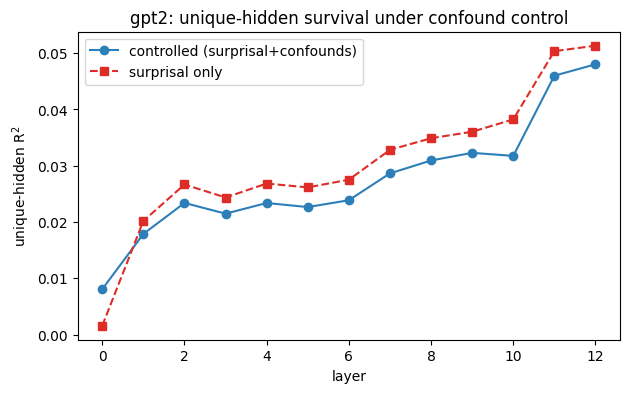
\includegraphics[width=0.65\linewidth]{figures/fig_confound_survival}
\caption{Unique-hidden survival under confound control (GPT-2). Solid blue: unique-hidden when
controlling for the full nuisance space (surprisal, entropy, word rate/length/frequency,
position). Dashed red: controlling for surprisal only. The two curves nearly coincide at every
layer---the positional and word-rate confounds of \citet{feghhi2024} absorb only a small slice
of unique-hidden---so the result is not explained by low-level stimulus signals.}
\label{fig:survival}
\end{figure}

\subsection{Robustness: per-subject aggregation matches pooled}
\label{sec:robust}
Because each voxel is fit independently in the encoding model, pooling voxels across subjects
never mixes subject signal in the \emph{fit}; pooled and per-subject estimates can differ only
in how voxels are weighted when averaged. Re-aggregating per-voxel unique-hidden by subject
(each of the $9$ subjects weighted equally) reproduces the pooled value for every model---e.g.\
GPT-2 $0.0480 \pm 0.0063$ (SEM) vs.\ pooled $0.0480$; Qwen2.5-1.5B $0.0700 \pm 0.0083$ vs.\
$0.0701$ (Figure~\ref{fig:persubject}). The central magnitude is therefore not an artifact of
joint-voxel pooling.

\begin{figure}[t]
\centering
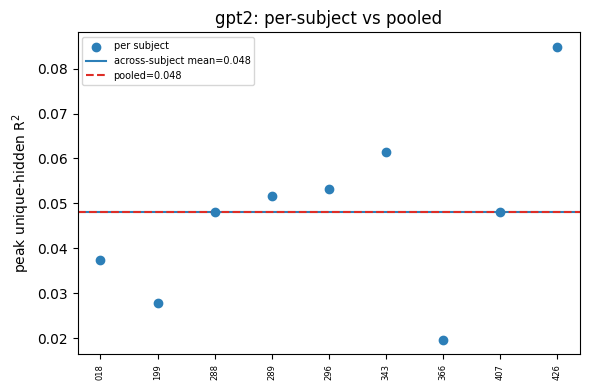
\includegraphics[width=0.55\linewidth]{figures/fig_per_subject}
\caption{Per-subject vs.\ pooled peak unique-hidden (GPT-2). Points are individual subjects; the
blue line is the across-subject mean (equal weight) and the dashed red line the pooled estimate.
They coincide, ruling out a voxel-pooling artifact.}
\label{fig:persubject}
\end{figure}

\subsection{Size: unique structure grows with scale within a family}
\label{sec:size}
Using the Pythia suite as a confound-free scaling axis (identical data and training order),
peak unique-hidden rises with scale and saturates near $1$B:
$0.032$ ($70$M) $\rightarrow 0.036$ ($160$M) $\rightarrow 0.053$ ($410$M)
$\rightarrow 0.061$ ($1$B) $\rightarrow 0.057$ ($1.4$B) (Figure~\ref{fig:scaling}, right).
This is a genuine five-point within-family trend rather than a single-step comparison. Across
families the relationship is \emph{not} monotonic in parameter count---well-trained small models
(GPT-2 $124$M: $0.048$; OPT-125M: $0.055$) exceed Pythia-160M, and the Qwen2.5 models sit above
the Pythia line at matched scale---indicating that architecture and training data, not parameter
count alone, govern the unique representational contribution. We therefore present cross-family
points for context only, not as a trend.

\begin{figure}[t]
\centering
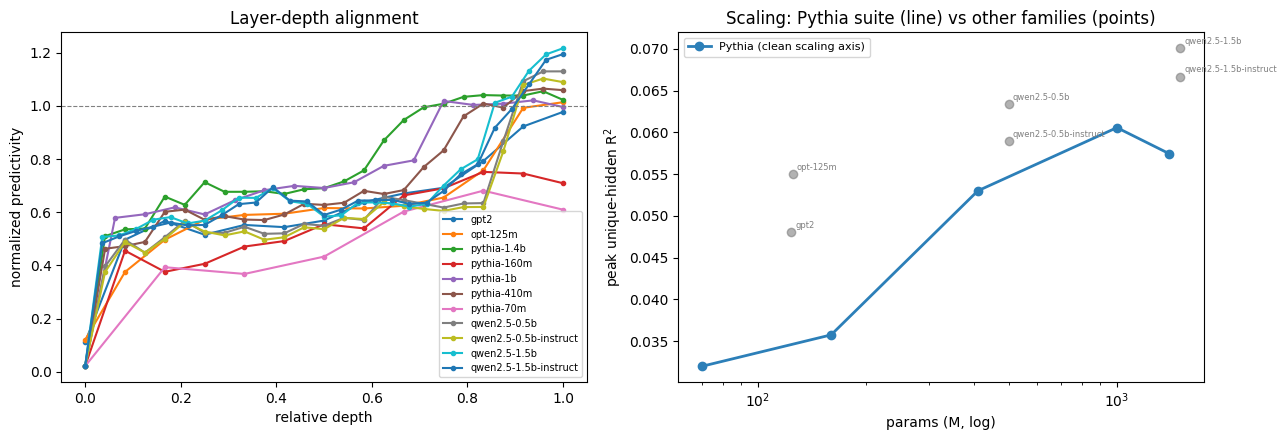
\includegraphics[width=\linewidth]{figures/fig_scaling}
\caption{\textbf{Left:} noise-ceiling-normalized predictivity vs.\ relative layer depth for all
eleven models; the dashed line marks the cross-subject ceiling. \textbf{Right:} peak
unique-hidden $R^2$ vs.\ parameter count. The Pythia suite (blue line) is the only confound-free
scaling axis (same data and step order) and rises with scale to $\sim$$1$B; cross-family models
(grey points) are shown for context, not as a trend.}
\label{fig:scaling}
\end{figure}

\subsection{Instruction tuning significantly reduces unique structure}
\label{sec:instruct}
We test two base/instruct pairs at different scales. At both, instruction tuning \emph{reduces}
peak unique-hidden, and a paired comparison across the $12{,}137$ shared voxels (each model at
its own peak layer) gives a strictly positive base$-$instruct difference
(Figure~\ref{fig:instruct}): Qwen2.5-0.5B, $0.0634 \rightarrow 0.0589$, mean difference
$+0.0056$ ($95\%$ bootstrap CI $[+0.0053, +0.0060]$); Qwen2.5-1.5B,
$0.0701 \rightarrow 0.0667$, $+0.0035$ ($[+0.0032, +0.0039]$). The effect is consistent in
direction and significant at both scales, though smaller at $1.5$B, so it is not a single-pair
idiosyncrasy. This runs opposite to \citet{aw2024}, who report that instruction tuning
\emph{raises} overall brain alignment. We stress that we do \emph{not} observe a rise even in
\emph{total} predictivity: on our cross-subject-normalized measure, instruction tuning lowers
norm $r$ slightly for both pairs as well ($1.13\rightarrow1.10$ and $1.22\rightarrow1.19$;
Table~\ref{tab:sweep}). The discrepancy is therefore one of dataset and metric scope, not a
contradiction internal to our pipeline: \citet{aw2024} aggregate a brain-alignment score across
several datasets under a different regression and ceiling protocol, whereas we measure
single-dataset (Pereira2018), noise-ceiling-normalized predictivity and the
unique-beyond-surprisal residual. Within our pipeline both total predictivity and the unique
residual decline modestly under instruction tuning; the robust, primary effect is the decline of
the unique structural residual, established by the paired voxel-level test above
(non-overlapping CIs at both scales).

\begin{figure}[t]
\centering
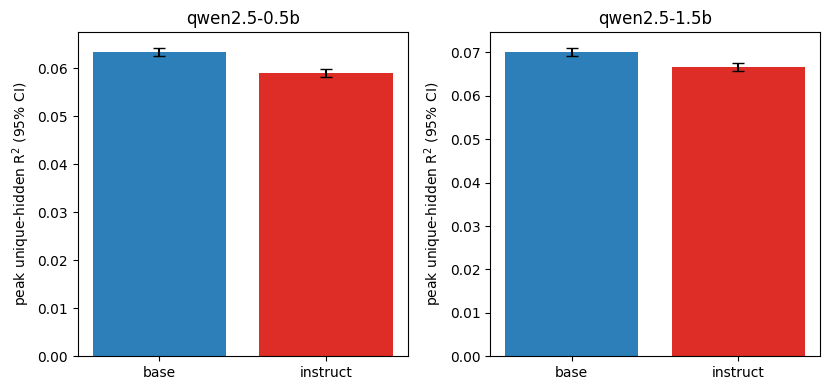
\includegraphics[width=0.8\linewidth]{figures/fig_instruct_pairs}
\caption{Peak unique-hidden $R^2$ (with $95\%$ CIs) for two base/instruct pairs. Instruction
tuning significantly reduces unique structure at both $0.5$B and $1.5$B, ruling out a
single-pair artifact.}
\label{fig:instruct}
\end{figure}

\begin{table}[t]
\caption{Model sweep on Pereira2018 ($384$-sentence experiment, last-token pooling,
cross-subject noise ceiling; stabilized LOO-GCV ridge). ``norm $r$'' is best-layer normalized
predictivity; ``unique$(H)$'' is the peak across layers with a $95\%$ voxel-bootstrap CI under
the \emph{full confound-controlled} nuisance space; ``\% ret.'' is the fraction retained relative
to the surprisal-only partition; $H{:}N$ is the unique-hidden:unique-nuisance ratio at the peak
layer. The two largest $H{:}N$ values (Pythia-1B, -1.4B) reflect a near-floor denominator, not a
larger numerator (Section~\ref{sec:core}). The released pipeline recomputes per-voxel raw $r$
(Section~\ref{sec:repro}); cross-model comparison should rely on the absolute, unnormalized peak
unique$(H)$ column rather than on norm $r$.}
\label{tab:sweep}
\centering
\begin{tabular}{lrrrrr}
\toprule
Model & Params & norm $r$ & peak unique$(H)$ [95\% CI] & \% ret. & $H{:}N$ \\
\midrule
Pythia-70M        & 70M   & 0.68 & 0.032 [.031,.033] & 92\% & 5$\times$ \\
GPT-2             & 124M  & 0.98 & 0.048 [.047,.049] & 94\% & 7$\times$ \\
OPT-125M          & 125M  & 1.01 & 0.055 [.054,.056] & 91\% & 7$\times$ \\
Pythia-160M       & 160M  & 0.75 & 0.036 [.035,.037] & 91\% & 7$\times$ \\
Pythia-410M       & 410M  & 1.07 & 0.053 [.052,.054] & 91\% & 8$\times$ \\
Qwen2.5-0.5B      & 500M  & 1.13 & 0.063 [.063,.064] & 95\% & 9$\times$ \\
Qwen2.5-0.5B-Inst & 500M  & 1.10 & 0.059 [.058,.060] & 96\% & 8$\times$ \\
Pythia-1B         & 1B    & 1.02 & 0.061 [.060,.061] & 92\% & 43$\times$ \\
Pythia-1.4B       & 1.4B  & 1.06 & 0.057 [.057,.058] & 91\% & 16$\times$ \\
Qwen2.5-1.5B      & 1.5B  & 1.22 & 0.070 [.069,.071] & 95\% & 14$\times$ \\
Qwen2.5-1.5B-Inst & 1.5B  & 1.19 & 0.067 [.066,.068] & 96\% & 13$\times$ \\
\bottomrule
\end{tabular}
\end{table}

\subsection{Representational geometry (RSA cross-check)}
\label{sec:rsa}
As a geometry-level cross-check independent of the linear encoding model, we correlate each
layer's representational dissimilarity matrix (RDM) with the brain RDM
(Figure~\ref{fig:geometry}). RSA scores are small and noisier than the encoding
results---peaking around $\rho \approx 0.04$--$0.05$---but are positive for the most predictive
models and broadly consistent with the encoding ordering, indicating the linear-predictivity
findings are not an artifact of the encoding mapping alone.

\begin{figure}[t]
\centering
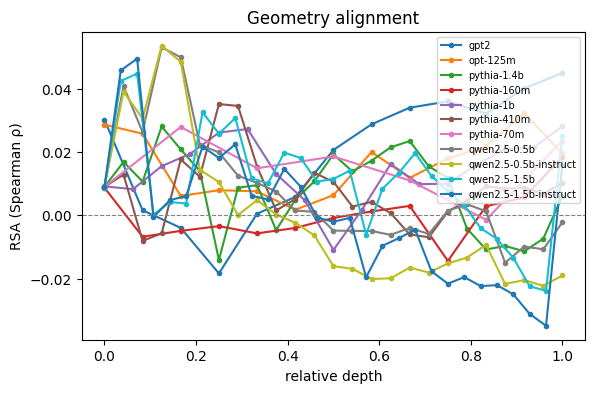
\includegraphics[width=0.65\linewidth]{figures/fig_geometry_all}
\caption{RSA (Spearman $\rho$ between model-layer and brain RDMs) vs.\ relative depth for all
eleven models. Scores are small but positive for the more predictive models, corroborating the
encoding-model results with a mapping-free measure.}
\label{fig:geometry}
\end{figure}

\section{Discussion and Limitations}
\label{sec:discussion}
Our central result---that hidden representations uniquely explain far more brain variance than a
\emph{confound-controlled} nuisance space, growing with depth and surviving the positional and
word-rate controls of \citet{feghhi2024}---supports a structural, rather than purely predictive
or confound-driven, account of LLM--brain alignment, while quantifying the (small but non-zero)
unique nuisance contribution. We state plainly that ``survives confound control'' means survival
of \emph{these} controls---the positional and word-rate signals of \citet{feghhi2024} together
with predictive entropy, word length, and frequency---and not confound-completeness: richer
positional, discourse, or symbolic-syntactic covariates (Limitations~iv--v) could absorb
additional variance.

\paragraph{Limitations.} (i) Our main sweep uses the $384$-sentence experiment; on the
independent $243$-sentence experiment ($6$ subjects, $8{,}031$ voxels) the core result already
replicates---GPT-2 peak unique$(H)=0.049$ [$.048,.050$] and Qwen2.5-0.5B $0.046$ [$.044,.047$],
both far exceeding unique-nuisance---and a full size/instruction-tuning sweep there is in
progress. (ii) Our cross-subject ceiling is
principled but not identical to the brain-score extrapolation ceiling; some normalized values
exceed $1$, indicating a conservative ceiling estimate, so we anchor cross-model comparison on
the absolute unique$(H)$ $R^2$ and release per-voxel raw $r$, rather than over-interpreting
normalized cross-model rankings. (iii) Confidence intervals are bootstrap over
voxels; a stimulus-level bootstrap is stronger and planned. (iv) Our positional confound uses
sentence position within its passage; finer positional and discourse covariates could absorb
slightly more variance. (v) Even an entropy-augmented surprisal is a coarse ``statistics'' side;
richer symbolic-syntactic predictors would further sharpen the ``structure'' side.

\section{Conclusion}
\label{sec:conclusion}
Framing the structure-versus-statistics debate as a \emph{confound-controlled}
variance-partitioning question yields a clear, reproducible answer on Pereira2018: alignment is
carried overwhelmingly by hidden representations beyond surprisal \emph{and} the positional and
word-rate confounds that otherwise dominate this dataset; this unique contribution grows with
scale within a controlled model family, is shaped by architecture and training across families,
matches per-subject and pooled estimates, and is significantly reduced by instruction tuning at
two scales. The full pipeline runs inference-only and is released for reproduction.

\section*{Reproducibility}
Code, configuration, and the experiment tracker are available at
\url{https://github.com/Sudarssan-N/LLMBrainAllignment}. All results use public models and the
public Pereira2018 release via \texttt{brain-score/language}; the single notebook
\texttt{notebooks/run\_experiments.ipynb} regenerates every number and figure end-to-end.

\bibliographystyle{plainnat}
\bibliography{references}

\end{document}
